
% Define a custom style for error bars on bars in PGFPlots
% This block should ideally be in your main document's preamble if used globally
\pgfplotsset{
    error bars/ybar error/.style={
        /pgfplots/error bars/y dir=both,
        /pgfplots/error bars/y explicit,
        /pgfplots/error bars/error mark options={
            rotate=90, % Ensure error bar caps are horizontal
            xshift=0pt % Adjust as needed
        }
    }
}

\begin{figure*}[!ht] % Use figure* for a wide figure spanning two columns
    \centering
    % Loop through each case size to create a subfigure

    \begin{subfigure}[b]{0.48\textwidth} % Adjust width as needed for 2x2 layout
        \centering
        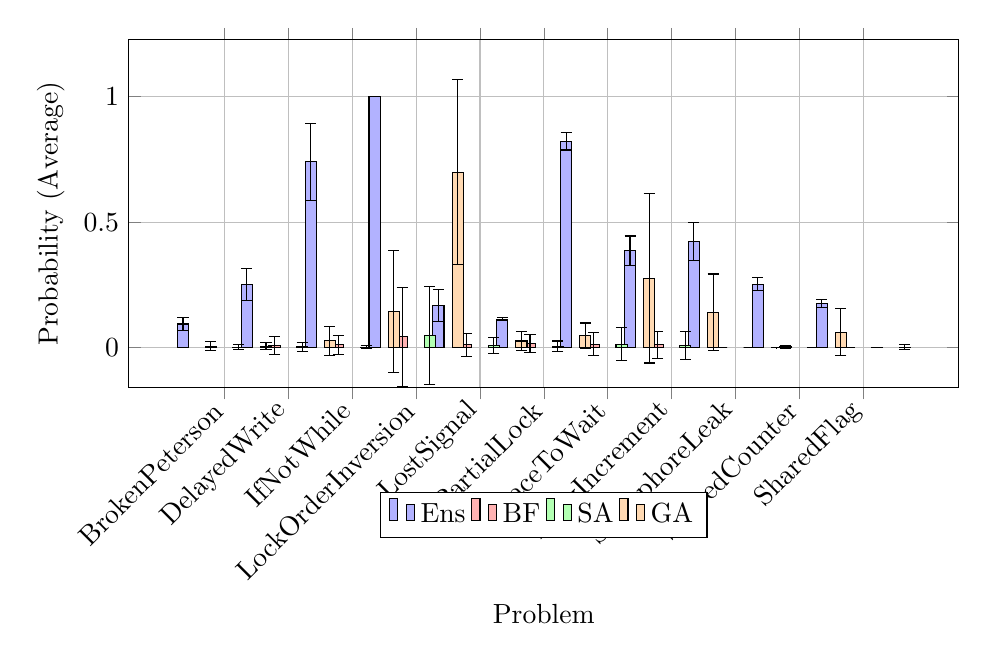
\begin{tikzpicture}
        \begin{axis}[
            ybar, % Bar plot type
            bar width=4pt, % Width of individual bars
            width=\textwidth, height=6cm, % Size of the axis environment
            ymin=0, % Start y-axis from 0
            xlabel={Problem},
            ylabel={Probability (Average)},
            xtick=data, % Use data points for x-ticks
            xticklabel style={rotate=45, anchor=east}, % Rotate x-labels
            enlargelimits=0.15, % Enlarge limits to give space around bars
            symbolic x coords={BrokenPeterson,DelayedWrite,IfNotWhile,LockOrderInversion,LostSignal,PartialLock,RaceToWait,RacyIncrement,SemaphoreLeak,SharedCounter,SharedFlag}, % Use problem names as symbolic x-coordinates
            % Legend style for the subfigure (will be hidden for all but the first)
            legend style={at={(0.5,-0.30)}, anchor=north,legend columns=-1},
            grid=both, % Show grid lines
        ]
            \addlegendentry{Ens}
            \addlegendentry{BF}
            \addlegendentry{SA}
            \addlegendentry{GA}
            \addplot[draw=black, fill=blue!30, error bars/ybar error, xshift=-6.0pt] coordinates { (BrokenPeterson,0.09358000000000001) +-(0,0.02435627564438588) (DelayedWrite,0.2512400000000001) +-(0,0.0646695083182362) (IfNotWhile,0.7401599999999999) +-(0,0.1529480850965248) (LockOrderInversion,1.0) +-(0,0.0) (LostSignal,0.16874) +-(0,0.06339439555477373) (PartialLock,0.11266) +-(0,0.005836584128213547) (RaceToWait,0.8224000000000001) +-(0,0.03505272995860693) (RacyIncrement,0.3852799999999999) +-(0,0.05935505067655488) (SemaphoreLeak,0.42225999999999997) +-(0,0.07566408308694297) (SharedCounter,0.25283999999999995) +-(0,0.025212047654618923) (SharedFlag,0.17656000000000002) +-(0,0.01580513995444494) };
            \addplot[draw=black, fill=red!30, error bars/ybar error, xshift=-2.0pt] coordinates { (BrokenPeterson,0.00578) +-(0,0.017645361302909165) (DelayedWrite,0.008539999999999999) +-(0,0.03643961177238925) (IfNotWhile,0.010860000000000002) +-(0,0.038050991566366224) (LockOrderInversion,0.042260000000000006) +-(0,0.19792132120556166) (LostSignal,0.01034) +-(0,0.04537715419072663) (PartialLock,0.01636) +-(0,0.03553713780350502) (RaceToWait,0.013600000000000001) +-(0,0.04670882449510248) (RacyIncrement,0.01098) +-(0,0.05437867604275838) (SemaphoreLeak,0.0) +-(0,0.0) (SharedCounter,0.0018999999999999998) +-(0,0.007211810041982016) (SharedFlag,0.0) +-(0,0.0) };
            \addplot[draw=black, fill=green!30, error bars/ybar error, xshift=2.0pt] coordinates { (BrokenPeterson,0.00168) +-(0,0.011022129873067886) (DelayedWrite,0.0031) +-(0,0.01774910173064817) (IfNotWhile,0.00106) +-(0,0.005246612123600352) (LockOrderInversion,0.04769999999999999) +-(0,0.196819636692468) (LostSignal,0.007540000000000002) +-(0,0.03217567213829449) (PartialLock,0.00434) +-(0,0.021483368032988132) (RaceToWait,0.01322) +-(0,0.06554054361342189) (RacyIncrement,0.00902) +-(0,0.056137037139267605) (SemaphoreLeak,0.0) +-(0,0.0) (SharedCounter,0.00012) +-(0,0.000848528137423857) (SharedFlag,0.0) +-(0,0.0) };
            \addplot[draw=black, fill=orange!30, error bars/ybar error, xshift=6.0pt] coordinates { (BrokenPeterson,0.004940000000000001) +-(0,0.013418552493484837) (DelayedWrite,0.02737999999999999) +-(0,0.05780434628105046) (IfNotWhile,0.1441) +-(0,0.2429957797567518) (LockOrderInversion,0.6988) +-(0,0.3679851372331357) (LostSignal,0.02605999999999999) +-(0,0.037282928193663634) (PartialLock,0.04738000000000001) +-(0,0.050279581606558855) (RaceToWait,0.27577999999999997) +-(0,0.3375984990052715) (RacyIncrement,0.14128) +-(0,0.15162440706009883) (SemaphoreLeak,4e-05) +-(0,0.000282842712474619) (SharedCounter,0.060439999999999994) +-(0,0.09386467897555328) (SharedFlag,0.0014000000000000002) +-(0,0.009899494936611667) };

        \end{axis}
        \end{tikzpicture}
        \caption{100 Test Cases} % Caption for the individual subfigure
        \label{fig:case_100}
    \end{subfigure}
    \hfill
    \begin{subfigure}[b]{0.48\textwidth} % Adjust width as needed for 2x2 layout
        \centering
        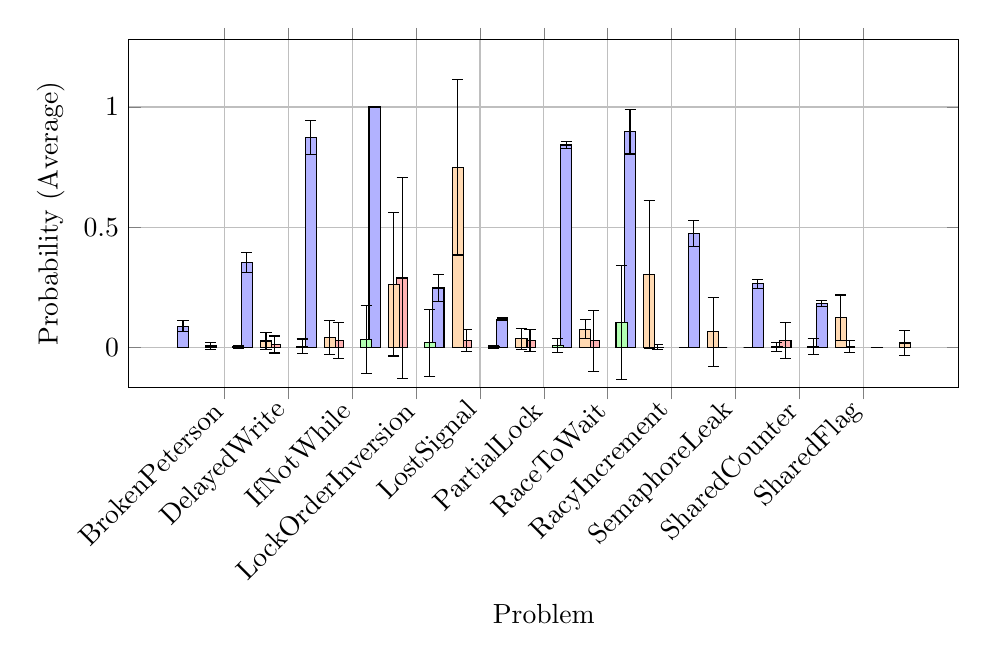
\begin{tikzpicture}
        \begin{axis}[
            ybar, % Bar plot type
            bar width=4pt, % Width of individual bars
            width=\textwidth, height=6cm, % Size of the axis environment
            ymin=0, % Start y-axis from 0
            xlabel={Problem},
            ylabel={Probability (Average)},
            xtick=data, % Use data points for x-ticks
            xticklabel style={rotate=45, anchor=east}, % Rotate x-labels
            enlargelimits=0.15, % Enlarge limits to give space around bars
            symbolic x coords={BrokenPeterson,DelayedWrite,IfNotWhile,LockOrderInversion,LostSignal,PartialLock,RaceToWait,RacyIncrement,SemaphoreLeak,SharedCounter,SharedFlag}, % Use problem names as symbolic x-coordinates
            % Legend style for the subfigure (will be hidden for all but the first)
            legend style={at={(0.5,-0.30)}, anchor=north,legend columns=-1},
            grid=both, % Show grid lines
        ]
            \addplot[draw=black, fill=blue!30, error bars/ybar error, xshift=-6.0pt] coordinates { (BrokenPeterson,0.08850000000000001) +-(0,0.02362742267029598) (DelayedWrite,0.3538400000000001) +-(0,0.04056708226216455) (IfNotWhile,0.8731800000000003) +-(0,0.0698355765717019) (LockOrderInversion,1.0) +-(0,0.0) (LostSignal,0.24739999999999998) +-(0,0.055892389317987325) (PartialLock,0.11707999999999999) +-(0,0.00580935206615776) (RaceToWait,0.8418800000000001) +-(0,0.015311247033285227) (RacyIncrement,0.8970599999999997) +-(0,0.09251991732616972) (SemaphoreLeak,0.47329999999999983) +-(0,0.053275276649126395) (SharedCounter,0.2646200000000001) +-(0,0.01746704185088042) (SharedFlag,0.1844000000000001) +-(0,0.012912578901116195) };
            \addplot[draw=black, fill=red!30, error bars/ybar error, xshift=-2.0pt] coordinates { (BrokenPeterson,0.00636) +-(0,0.014992188442175954) (DelayedWrite,0.01272) +-(0,0.03538824894319167) (IfNotWhile,0.02963999999999999) +-(0,0.07476350741382004) (LockOrderInversion,0.28888) +-(0,0.41910929069995617) (LostSignal,0.02881999999999999) +-(0,0.046706941318683456) (PartialLock,0.03016) +-(0,0.045241465538614384) (RaceToWait,0.0277) +-(0,0.1265817877089427) (RacyIncrement,0.0014000000000000002) +-(0,0.009615039240265051) (SemaphoreLeak,0.0) +-(0,0.0) (SharedCounter,0.02846) +-(0,0.07467540916991267) (SharedFlag,0.00434) +-(0,0.023893137944111204) };
            \addplot[draw=black, fill=green!30, error bars/ybar error, xshift=2.0pt] coordinates { (BrokenPeterson,0.00214) +-(0,0.007122857715890184) (DelayedWrite,0.005540000000000001) +-(0,0.02998108927783836) (IfNotWhile,0.03268) +-(0,0.14068439711580216) (LockOrderInversion,0.0197) +-(0,0.13930003589374987) (LostSignal,0.00198) +-(0,0.006640906011461179) (PartialLock,0.00946) +-(0,0.028718343707569947) (RaceToWait,0.105) +-(0,0.2378197739843329) (RacyIncrement,0.0002) +-(0,0.0014142135623730952) (SemaphoreLeak,0.0) +-(0,0.0) (SharedCounter,0.00486) +-(0,0.034221374153876286) (SharedFlag,0.0) +-(0,0.0) };
            \addplot[draw=black, fill=orange!30, error bars/ybar error, xshift=6.0pt] coordinates { (BrokenPeterson,0.027100000000000003) +-(0,0.035932618346350566) (DelayedWrite,0.04189999999999999) +-(0,0.07140035156833356) (IfNotWhile,0.2623) +-(0,0.2974692060893506) (LockOrderInversion,0.7486) +-(0,0.363911740813677) (LostSignal,0.03651999999999999) +-(0,0.04399918366589665) (PartialLock,0.07650000000000003) +-(0,0.04008880448327132) (RaceToWait,0.30363999999999997) +-(0,0.3084776815265572) (RacyIncrement,0.06544) +-(0,0.1440072503843654) (SemaphoreLeak,0.00382) +-(0,0.018910843450253612) (SharedCounter,0.12433999999999999) +-(0,0.09413724457581352) (SharedFlag,0.018860000000000002) +-(0,0.052063936360860714) };

        \end{axis}
        \end{tikzpicture}
        \caption{500 Test Cases} % Caption for the individual subfigure
        \label{fig:case_500}
    \end{subfigure}

    \par\vspace{\baselineskip} % Add some vertical space between rows

    \begin{subfigure}[b]{0.48\textwidth} % Adjust width as needed for 2x2 layout
        \centering
        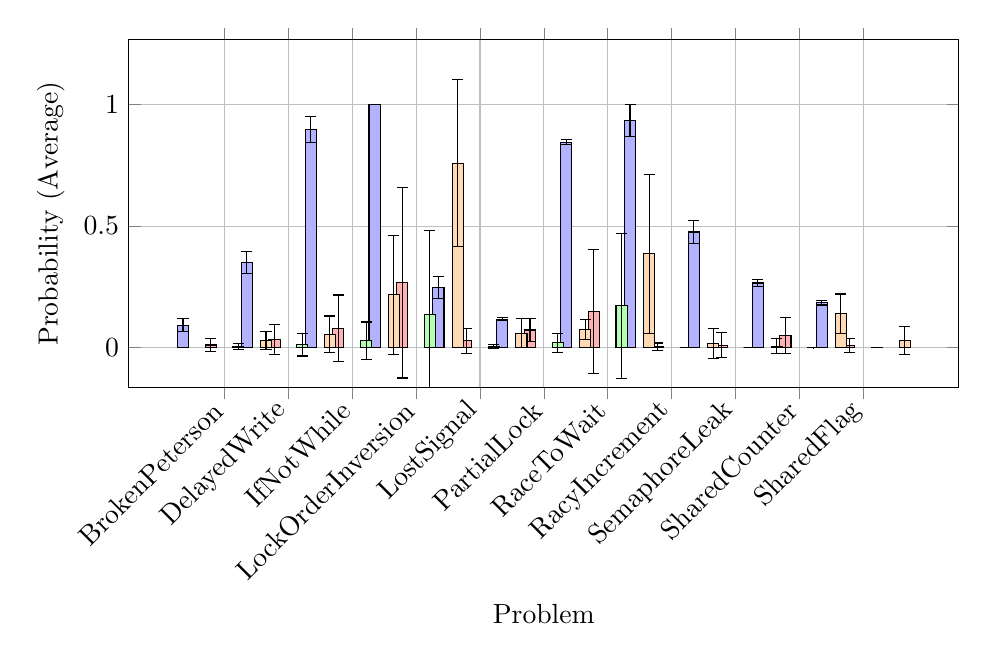
\begin{tikzpicture}
        \begin{axis}[
            ybar, % Bar plot type
            bar width=4pt, % Width of individual bars
            width=\textwidth, height=6cm, % Size of the axis environment
            ymin=0, % Start y-axis from 0
            xlabel={Problem},
            ylabel={Probability (Average)},
            xtick=data, % Use data points for x-ticks
            xticklabel style={rotate=45, anchor=east}, % Rotate x-labels
            enlargelimits=0.15, % Enlarge limits to give space around bars
            symbolic x coords={BrokenPeterson,DelayedWrite,IfNotWhile,LockOrderInversion,LostSignal,PartialLock,RaceToWait,RacyIncrement,SemaphoreLeak,SharedCounter,SharedFlag}, % Use problem names as symbolic x-coordinates
            % Legend style for the subfigure (will be hidden for all but the first)
            legend style={at={(0.5,-0.30)}, anchor=north,legend columns=-1},
            grid=both, % Show grid lines
        ]
            \addplot[draw=black, fill=blue!30, error bars/ybar error, xshift=-6.0pt] coordinates { (BrokenPeterson,0.09214) +-(0,0.025561458551211565) (DelayedWrite,0.35024) +-(0,0.044546036723316806) (IfNotWhile,0.8967399999999999) +-(0,0.05391861213619911) (LockOrderInversion,1.0) +-(0,0.0) (LostSignal,0.24705999999999992) +-(0,0.044134492966247864) (PartialLock,0.11654) +-(0,0.005610522184580812) (RaceToWait,0.84538) +-(0,0.011193821181931633) (RacyIncrement,0.9343999999999997) +-(0,0.06678414818637422) (SemaphoreLeak,0.47580000000000006) +-(0,0.04651223231690821) (SharedCounter,0.26558) +-(0,0.013806372382611837) (SharedFlag,0.18507999999999997) +-(0,0.010201720543164098) };
            \addplot[draw=black, fill=red!30, error bars/ybar error, xshift=-2.0pt] coordinates { (BrokenPeterson,0.01034) +-(0,0.026119513387347717) (DelayedWrite,0.03183999999999999) +-(0,0.0612166977354435) (IfNotWhile,0.07875999999999998) +-(0,0.13734517219957393) (LockOrderInversion,0.26617999999999997) +-(0,0.391723491087001) (LostSignal,0.027759999999999993) +-(0,0.05136565993354084) (PartialLock,0.07204000000000002) +-(0,0.04659857228258722) (RaceToWait,0.1467) +-(0,0.25517710936300136) (RacyIncrement,0.00364) +-(0,0.014930806394560098) (SemaphoreLeak,0.01008) +-(0,0.051927280392675995) (SharedCounter,0.04988000000000001) +-(0,0.07434767745435726) (SharedFlag,0.008020000000000001) +-(0,0.028689392194499272) };
            \addplot[draw=black, fill=green!30, error bars/ybar error, xshift=2.0pt] coordinates { (BrokenPeterson,0.00482) +-(0,0.013466041946848585) (DelayedWrite,0.01098) +-(0,0.04587538133078458) (IfNotWhile,0.0279) +-(0,0.07733949805360565) (LockOrderInversion,0.13752) +-(0,0.3446175780514407) (LostSignal,0.00254) +-(0,0.00823682621659878) (PartialLock,0.019639999999999998) +-(0,0.03980552725439019) (RaceToWait,0.17170000000000002) +-(0,0.2980828024943021) (RacyIncrement,0.0) +-(0,0.0) (SemaphoreLeak,0.0) +-(0,0.0) (SharedCounter,0.0001) +-(0,0.0007071067811865476) (SharedFlag,0.0) +-(0,0.0) };
            \addplot[draw=black, fill=orange!30, error bars/ybar error, xshift=6.0pt] coordinates { (BrokenPeterson,0.02927999999999999) +-(0,0.03774297610016942) (DelayedWrite,0.05528) +-(0,0.0745629551836184) (IfNotWhile,0.21658000000000002) +-(0,0.24518748261820603) (LockOrderInversion,0.75796) +-(0,0.34380760875340605) (LostSignal,0.0593) +-(0,0.06085219631137701) (PartialLock,0.07560000000000001) +-(0,0.041043033662789774) (RaceToWait,0.38526000000000005) +-(0,0.3280727775158109) (RacyIncrement,0.017200000000000003) +-(0,0.061506594967448786) (SemaphoreLeak,0.0057599999999999995) +-(0,0.03032245749558285) (SharedCounter,0.13946) +-(0,0.08104778383957281) (SharedFlag,0.02836) +-(0,0.05685669777284514) };

        \end{axis}
        \end{tikzpicture}
        \caption{1100 Test Cases} % Caption for the individual subfigure
        \label{fig:case_1100}
    \end{subfigure}
    \hfill
    \begin{subfigure}[b]{0.48\textwidth} % Adjust width as needed for 2x2 layout
        \centering
        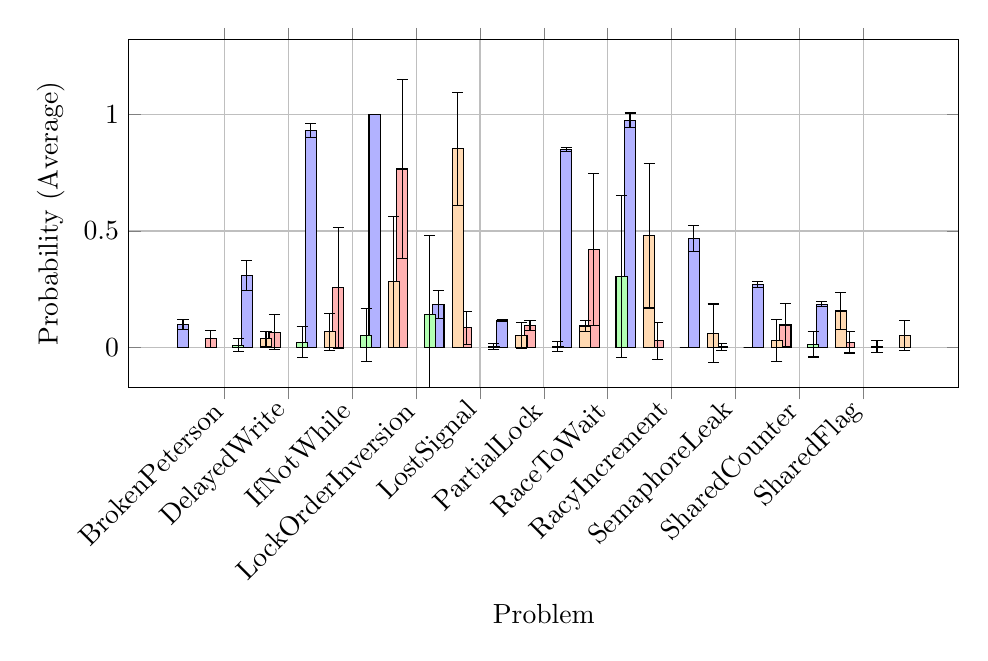
\begin{tikzpicture}
        \begin{axis}[
            ybar, % Bar plot type
            bar width=4pt, % Width of individual bars
            width=\textwidth, height=6cm, % Size of the axis environment
            ymin=0, % Start y-axis from 0
            xlabel={Problem},
            ylabel={Probability (Average)},
            xtick=data, % Use data points for x-ticks
            xticklabel style={rotate=45, anchor=east}, % Rotate x-labels
            enlargelimits=0.15, % Enlarge limits to give space around bars
            symbolic x coords={BrokenPeterson,DelayedWrite,IfNotWhile,LockOrderInversion,LostSignal,PartialLock,RaceToWait,RacyIncrement,SemaphoreLeak,SharedCounter,SharedFlag}, % Use problem names as symbolic x-coordinates
            % Legend style for the subfigure (will be hidden for all but the first)
            legend style={at={(0.5,-0.30)}, anchor=north,legend columns=-1},
            grid=both, % Show grid lines
        ]
            \addplot[draw=black, fill=blue!30, error bars/ybar error, xshift=-6.0pt] coordinates { (BrokenPeterson,0.09764000000000005) +-(0,0.021889108278421894) (DelayedWrite,0.30963999999999997) +-(0,0.06352944359965405) (IfNotWhile,0.9312800000000001) +-(0,0.03153361665892188) (LockOrderInversion,1.0) +-(0,0.0) (LostSignal,0.18442) +-(0,0.061742748066274965) (PartialLock,0.11600000000000002) +-(0,0.004412412917565857) (RaceToWait,0.85004) +-(0,0.00803807266979455) (RacyIncrement,0.9746399999999998) +-(0,0.03127609767401115) (SemaphoreLeak,0.4676600000000001) +-(0,0.05507383170595142) (SharedCounter,0.26982) +-(0,0.012981446729223724) (SharedFlag,0.18604000000000007) +-(0,0.010969270621111676) };
            \addplot[draw=black, fill=red!30, error bars/ybar error, xshift=-2.0pt] coordinates { (BrokenPeterson,0.03696) +-(0,0.03616456716687409) (DelayedWrite,0.06592000000000002) +-(0,0.07493176215458858) (IfNotWhile,0.2568999999999999) +-(0,0.25964891916680466) (LockOrderInversion,0.7658200000000001) +-(0,0.38216113120525713) (LostSignal,0.08453999999999998) +-(0,0.07010057206672171) (PartialLock,0.09421999999999998) +-(0,0.02239742149882263) (RaceToWait,0.42052) +-(0,0.32527603599379523) (RacyIncrement,0.028259999999999997) +-(0,0.0807275109266238) (SemaphoreLeak,0.0024600000000000004) +-(0,0.016550738315117854) (SharedCounter,0.09643999999999997) +-(0,0.0937654825310771) (SharedFlag,0.0233) +-(0,0.046839826939850046) };
            \addplot[draw=black, fill=green!30, error bars/ybar error, xshift=2.0pt] coordinates { (BrokenPeterson,0.0102) +-(0,0.02820840806770715) (DelayedWrite,0.022019999999999998) +-(0,0.0665605417216966) (IfNotWhile,0.05278000000000001) +-(0,0.11345093158520568) (LockOrderInversion,0.14114000000000002) +-(0,0.33817764984863036) (LostSignal,0.0041600000000000005) +-(0,0.013213104194283024) (PartialLock,0.0054) +-(0,0.02160876617278747) (RaceToWait,0.3041) +-(0,0.3473931637267516) (RacyIncrement,0.0) +-(0,0.0) (SemaphoreLeak,0.0) +-(0,0.0) (SharedCounter,0.01322) +-(0,0.05367030494279924) (SharedFlag,0.00376) +-(0,0.02658721497261419) };
            \addplot[draw=black, fill=orange!30, error bars/ybar error, xshift=6.0pt] coordinates { (BrokenPeterson,0.0372) +-(0,0.03197128813961243) (DelayedWrite,0.06717999999999999) +-(0,0.07964274567577082) (IfNotWhile,0.28156000000000003) +-(0,0.2817782570079688) (LockOrderInversion,0.8522799999999999) +-(0,0.24199216043972524) (LostSignal,0.053119999999999994) +-(0,0.05591525657964334) (PartialLock,0.09246000000000003) +-(0,0.023190612104813282) (RaceToWait,0.4794599999999999) +-(0,0.3098583751539747) (RacyIncrement,0.060360000000000004) +-(0,0.1264395895118233) (SemaphoreLeak,0.0305) +-(0,0.08955200290607575) (SharedCounter,0.15668000000000004) +-(0,0.07888597816481965) (SharedFlag,0.05074000000000001) +-(0,0.0639584718583002) };

        \end{axis}
        \end{tikzpicture}
        \caption{3900 Test Cases} % Caption for the individual subfigure
        \label{fig:case_3900}
    \end{subfigure}

    \caption{Performance of different optimization methods across various problem instances for different test case sizes. Each subplot shows the average probability of success with standard deviation for Ensemble (Ens), Brute Force (BF), Simulated Annealing (SA), and Genetic Algorithm (GA) methods.}
    \label{fig:all_method_performance}
\end{figure*}
